\documentclass[../ClipsManualeUtente.tex]{subfiles}

\begin{document}

\section{Altre funzionalità dell'applicazione}
	Nella sezione seguente vengono raccolte tutte le istruzioni necessarie per poter usufruire pienamente di tutte le altre funzionalità a supporto della navigazione offerte dall'applicazione CLIPS.
	
	\newpage
	\subsection{Esplora luoghi nelle vicinanze}
		L'applicazione è in grado di individuare la posizione approssimata dello smartphone all'interno dell'edificio.
		È possibile visualizzare una lista delle aree di interesse attorno alla posizione in cui si è, per visualizzare ciò:
		\begin{enumerate}
		\item attiva il \textbf{bluetooth};
		\item attiva una \textbf{connessione dati} oppure una \textbf{connessione Wi-fi} e assicurati che lo smartphone sia connesso ad Internet;
		\item \textbf{avvia l'applicazione} selezionando l'icona 
\includegraphics[scale=0.4]{img/LogoApp};
		\item assicurati di essere in un \textbf{edifico supportato} dall'applicazione. Per assicurarsi di ciò basta accertarsi che dalla schermata principale dell'applicazione siano visibili le informazioni dell'edificio;
		
		\begin{framed}
			\textbf{Nota:} solo per i dispositivi con \textbf{Android `Marshmallow' 6.0} - il \textbf{GPS} dello smartphone deve essere \textbf{attivato} prima di avviare l'applicazione.
		\end{framed}
		
		\item selezione il pulsante segnalato in figura \ref{fig:PulsanteEsplora}.
		\end{enumerate}
		
		\begin{figure} [h]
			\centering
			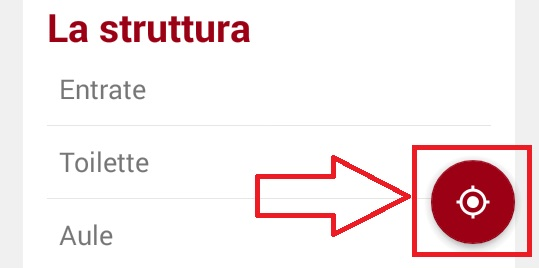
\includegraphics[scale=0.3]{img/PulsanteEsplora}
			\caption{Pulsante per accedere alla lista di aree d'interesse vicine}
			\label{fig:PulsanteEsplora}
		\end{figure}
		
		\begin{figure} [h]
			\centering
			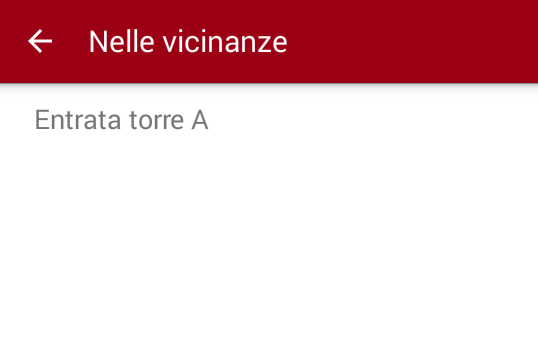
\includegraphics[scale=0.3]{img/ListaNearbyPoi}
			\caption{Lista di possibili aree d'interesse ottenuta dopo la procedura}
		\end{figure}
		
\iffalse % non implementata e non stampata nel pdf
	\newpage
	\subsection{Preferenze}
		È possibile configurare la navigazione attraverso l'impostazione di determinate preferenze. Tali preferenze impatteranno nel calcolo del percorso nella navigazione.
		Le preferenze disponibili sono:
			\begin{itemize}
				\item ???;
				\item ???.
			\end{itemize}
		
		Per impostare le proprie preferenze:
		\begin{enumerate}
			\item apri il menu dell'applicazione selezionando l'icona $\equiv$;
			\item seleziona \textbf{Preferenze};
			\item seleziona ??? per ???;
			\item seleziona ??? per ???.
		\end{enumerate}

	\begin{framed} 
	\textbf{Nota:} una volta impostate le preferenze, esse saranno attive solo dalla prossima navigazione avviata.
	\end{framed}
\fi	
	%\newpage
	%\subsection{Gestire le mappe}	
		
		
	\newpage
	\subsection{Area sviluppatore}
		L'applicazione rende disponibile a chi è in possesso della \textbf{password sviluppatore} un'area per poter accedere ai file log creati dall'applicazione durante il suo utilizzo.
		
		\begin{framed}
			\textbf{Nota:} questa funzionalità è creata specificatamente per chi dovrà effettuare dei test sul campo dell'applicazione e raccogliere dati sull'applicazione. Il normale utilizzo dell'applicazione \textbf{non richiede} l'uso di questa funzionalità.
		\end{framed}
		
		Tale materiale ha lo scopo di fornire tutte le informazioni ritenute utili sugli ultimi utilizzi della  funzionalità di navigazione. Questo può essere d'aiuto per espandere il suo potenziale o migliorare la mappatura dell'edificio con i dispositivi beacon.
		
		Per accedere all'area sviluppatore:
		\begin{enumerate}
			\item apri il menu dell'applicazione selezionando l'icona $\equiv$;
			\item seleziona \textbf{Area sviluppatore}; %figure inline 
			\item inserisci la \textbf{password sviluppatore}, ti verrà mostrata la lista dei file log in ordine di data e ora;
			\item seleziona il log di interesse per visualizzarlo; 
		\end{enumerate}

\end{document}